\documentclass[paper=letter]{article}

%%% Custom headers/footers (fancyhdr package)
\usepackage[backend=bibtex,style=numeric-comp]{biblatex}
\bibliography{bib.bib}
\usepackage{graphicx}
\usepackage{fancyhdr}
\usepackage{comment}
\pagestyle{fancyplain}
\fancyhead{}											% No page header
\fancyfoot[L]{}											% Empty 
\fancyfoot[C]{}											% Empty
\fancyfoot[R]{\thepage}									% Pagenumbering


\title{Performance Evaluation of Debian Linux on a Rasberry Pi}
\author{David Lisuk, Josh Marxen}
\date{\today}


%%% Begin document
\begin{document}
\maketitle
\section{Introduction}
The Rasberry Pi is a single board computer availible for under \$50 which is capable of running Linux distributions made for the ARM architecture.  
Originally targeted as an embedded computing learning aid, it has taken the world by storm with where an enthusiast community sprung up and utilized it for media centers, simple servers, robotics control boards, etc.
In this project, we obtain a performance profile of the Rasberry Pi model B computer, the flag ship ``full featured'' model.

Our team consists of Joshua Marxen and David Lisuk. 
David primarily did disk and memory experiments while Josh primarily did OS Services and Network.
However, both members contributed to all sections and the work distribution was approximately even.

Our compiler is gcc version 4.8.3, as implemented in the Raspbian linux operating system.
We disabled any compiler optimizations by compiling with the -O0 flag.
By analyzing the generated assembly code, we have found this optimization level to generate code close to the expected behavior and thus anticipate predictions to line up with measurements.

We evaluate the performance of 4 distinct hardware groups: CPU and OS Services, Memory, Network, and Disk.
For the rest of this paper, we first describe the Pi's hardware and software stack.
Then we describe our experiments by describing the general methodology then each of our four hardware groups separately.
\section{Machine Description}

To run our experiments we used a Raspberry Pi model B single board computer.   
This is a simple ARM 6 based computer which is availible for under \$50.
We run a Debian derivative on it for all performance measurements.
See table \ref{tbl:specs} for details on the hardware specs of the machine.

\begin{table}[h]
\label{tbl:specs}
\centering
\begin{tabular}{|l|l|}
\hline
                     & Documentation            \\ \hline
\multicolumn{2}{|c|}{\textbf{CPU}}              \\ \hline
Type                 & ARM 6 Compatible         \\ \hline
Model                & ARM1176JZF-S             \\ \hline
Cycle Time           & 1.4ns                    \\ \hline
L1 Cache             & 32KB (Ins+Data)          \\ \hline
L2 Cache             & 12KB (CPU+GPU)           \\ \hline
\multicolumn{2}{|c|}{\textbf{Memory}}           \\ \hline
Size                 & 512MB(CPU+GPU)           \\ \hline
Bus                  & DDR2                     \\ \hline
\multicolumn{2}{|c|}{\textbf{IO Bus}}           \\ \hline
Speed                & Unknown                  \\ \hline
\multicolumn{2}{|c|}{\textbf{Disk}}             \\ \hline
Type                 & Class 4 SD Card          \\ \hline
Size                 & 16GB                     \\ \hline
\multicolumn{2}{|c|}{\textbf{Network Card}}     \\ \hline
Speed                & 100MBPS                  \\ \hline
\multicolumn{2}{|c|}{\textbf{Operating System}} \\ \hline
Type                 & Linux                    \\ \hline
Distribution       & Raspbian(Debian)\\ \hline
Version             & Wheezy\\ \hline
Kernel Version  & 3.12.30+ \\\hline
\end{tabular}
\caption{Table of specs for the Rasberry Pi Model B\cite{infosheet}\cite{rpicomp}\cite{elinux}}
\end{table}

\newpage

\section{Experiments}
We developed a general wrapper program which calls an experiment specific inlined function.
This allows many of our experiments to share the number of running times, the statistic computation code and other things.
The basic code is shown below.

\begin{verbatim}
void setup();
void teardown();
unsigned long measure();

int main(void){
  int trial;
  unsigned int delta; // measurement

  df = fopen(exp_file_data_name, "w");

  setup(); // initialize environment for experiment
  for(trial = 0; trial < MAX_N; ++trial) {
    delta = measure();
    fprintf(df, "%ul\n", delta);
  }
  teardown();
  fclose(df);
}
\end{verbatim}

\noindent The {\tt setup}, {\tt teardown}, and {\tt measure} functions are implemented separately for each experiment. {\tt setup} sets up the environment necessary to run the experiment, and {\tt teardown} handles any cleaning up that needs to be done afterwards. {\tt measure} returns the measurement for each trial. We will give approximate c code for each of these experiments, but some details may be missing. We will include full code for each experiment in our final report.
\newline
\newline
Not all of the experiments were able to make use of this framework. We will explicitly identify which experiments these were in the report. Unless otherwise stated, assume that an experiment made use of this framework. Also, for those experiments that did use this framework, not all needed to implement the {\tt setup} and {\tt teardown} methods. Pseudocode for these will only be given when the experiment needed these.
\newline
\newline
Each datapoint is collected and written to an output file for offline processing.

\subsubsection{Computing Results}

\noindent We run each test 4978 times and report mean/standard deviation. We first take 5000 measurements, but then exclude the first 2 trials, as well as the highest 20 datapoints, before calculating the mean and variance. This is done to exclude inaccurate data collected as the experiment ``warms up" (ie, loads relevant pages into memory, code and data into L1 cache, etc.), as well as gross outliers from context switches and other uncontrollable interferences.

\subsubsection{Getting Time}
All time measurements in this report are in terms of cycles. Each cycle takes approximately 1.4 ns. We used two macros, {\tt reset} and {\tt GET\_HIGH}, to reset and read the cycle counter into a variable, respectively.

\subsubsection{Compilation}
We use gcc version 4.8.3 with the flag -O0 to prevent optimization.

\newpage

\subsection{CPU, Scheduling, and OS Services}
\subsubsection{Measurement Overhead}The first experiment measures the number of cycles passed between resetting the instruction counter and then reading it.
This time is the overhead associated with measuring and will be overhead for all experiments.

This experiment executes the {\tt RESET} macro and then the {\tt GET\_HIGH} macro on the next experiment.
The {\tt RESET} sets the clocks to 0 and then runs the serializing instruction to prevent OOO execution.
Since the serializing instruction and clocking will be pipelined one cycle will pass after the zeroing.
The {\tt GET\_HIGH} executes the serializing instruction (4 cycles from issue to execution), loads the destination variable from memory to a register(3 cycles according to documentation), then copies from the counter register to the variable register (4 cycles from start to register read due to pipeline).
After the register read the remaining work (transferring variable from register back into memory) will be outside of the measured time.
Thus we expect 12 cycles to pass from zeroing the counter till reading the counter.

Our experimental results found a mean time of 11 cycles with a standard deviation of 0.
This is one cycle shorter than our prediction.
It is probable that the destination reading and the counter copying will be pipelined so the copy takes is fetched while the memory is being read. 


\newpage

\subsubsection{Procedure Call Overhead}The next experiment we ran was to measure the amount of time it takes to run a procedure of 0-7 integer parameters and 1 returned integer.

Thus we implement experiment functions of this form: 
\begin{verbatim}
unsigned function(unsigned x_1, unsigned x_2){
  return 0;
}

static inline unsigned long execute(){
  return function(1, 2);
}
\end{verbatim}

To execute the procedure we have to load the arguments to registers, add the return pointer to the stack and then move the instruction pointer twice(there/back).
We suspect there are about 10 instructions per procedure call with 2 additional per parameter.  Most of these instructions deal with memory and thus will take a couple cycles each.  Thus we suspect about 20 cycles + 6 cycles per parameter.


\begin{figure}[h]
\centering
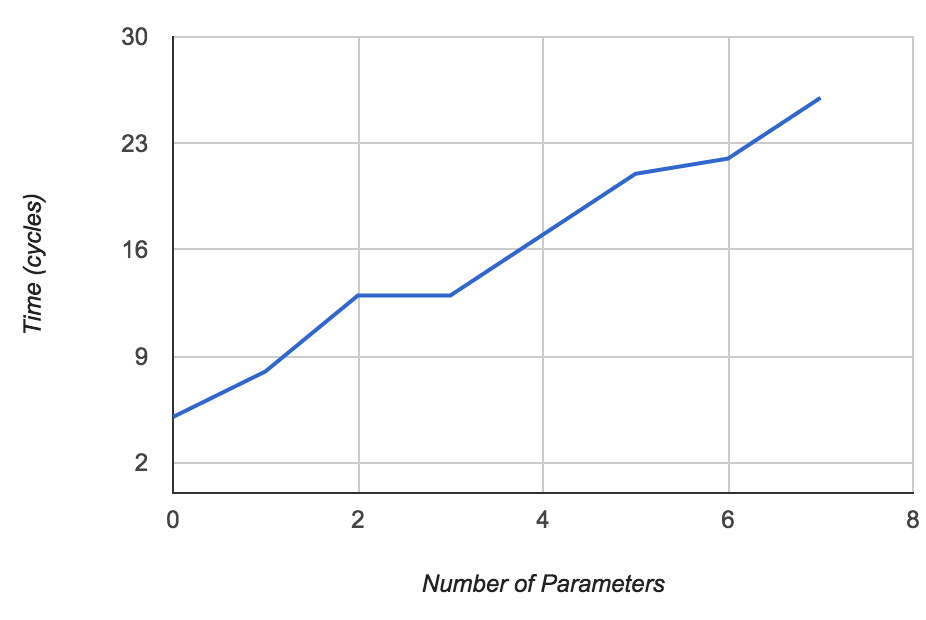
\includegraphics[scale=.5]{experiments/exp_1_2_fig.png}
\caption{Mean execution time vs number of parameters.  Overhead time included for comparison.  The standard deviation for all experiments was under 1 ns}
\end{figure}

There was a ~15 cycle overhead for procedure calls over the do nothing overhead.  Thus we were pretty close in our expected additional overhead for procedure calls.  There is also a strong linear relationship between number of procedure arguments and the time taken.  By performing a linear regression we get 4.2 ns additional cost per argument or about 3  additional cycles per parameter.

\newpage

\subsubsection{System Call Overhead}The third experiment we ran was to measure the amount of time taken by making an operating system call.
To do this we wish to execute a call which will do very little without being cached.  
We decided to use the {\tt getcpu} system call.
\newline
\newline
We implement this experiment as follows: 
\begin{verbatim}
unsigned long measure(){
  int rc;
  GET_HIGH(start);
  rc = syscall(SYS_getcpu);
  GET_HIGH(end);
  return end - start;
}
\end{verbatim}

We expect this to be about two orders of magnitude larger than the equivalent procedure call overhead, since we have to switch to the OS, do some work, and then switch back to our user program.  We take the sum of the procedure call overhead for a single argument and the overhead for returning from a function, and multiply by 100, to get $(19+16) \times 100 = 2500$ cycles.

The results of the experiment are"

\begin{table}[h]
\centering
\begin{tabular}{|c|c|}\hline
Mean & 2111 cycles \\
SD & 165 cycles\\\hline
\end{tabular}
\end{table}

This is roughly what we predicted, though we were off by about 3 standard deviations.

\newpage

\subsubsection{Task Creation Time}In the fourth experiment, we measure the time of task creation, both for ordinary processes and for kernel threads, and compare them.

To measure ordinary process creation time, we created a recursive program.
The basic idea is that the program relaunches itself using the {\tt excv} function.  
To ensure the program runs exactly 100 times, the program passes an argument {\tt trial} which is assumed to be 0 on first run and is incremented each re run.
Before recursing, the program resets the processor cycle counter to 0 and then the first thing the new process does is check the processor cycle counter.
This cycle count measures how many cycles occured between the {\tt excv} call and the first line of execution for the new process.
Thus we measure the time to create the new process.

To measure kthread creation time, we developed a kernel module and load it using insmod.
Upon loading, the loops 100 times, each time resting the cycle counter, starting a thread, and within the thread printing the value of the cycle counter.
To ensure the thread runs immediately (since we have a single core cpu), the module's main thread is told to sleep briefly after the thread is created.

The results of these two experiments are tabulated in Table \ref{tab:exp1_4}.
As you can see it takes about 3 million cycles to launch a process and 170k cycles to launch a kernel thread.
This is in line with expectations of a process taking significantly longer than a thread.

\begin{table}
\begin{tabular}{|c|c|c|}\hline
& Mean & Standard Deviation \\\hline
Process &  3100000 & 193338 \\
Kthread & 170000 & 72571 \\\hline
\end{tabular}
\caption{Results of process creation experiment}\label{tab:exp1_4}
\end{table}

\newpage

\subsubsection{Context Switch Time}In this experiment, we measure the time taken for a context switch to occur, both for ordinary processes and kernel threads. 

To measure process context switch, our program forks a child process and creates two blocking pipes between the two.
The parent writes and the child reads from pipe 1 and the opposite for pipe 2.
To measure performance, the parent sends a message to child, forcing a context switch.
The child then resets the instruction counter and sends a message to the parent, forcing a second context switch.
The parent prints the instruction counter.
This process cycles 100 times to get sufficient measurements.

To measure kernel context switching we developed a kernel module which spawns a single separate kthread and then force 100 context switches back and forth and measure the switching time.
Since kernel modules cannot use libc and thus piping, we had to get creative in forcing context switches. 
We utilize a single mutex lock which is locked by the child and unlocked by the parent.
Initially the lock is locked and the child thread is created and waits since it tries to lock the locked lock.
The parent then resets the process counter, unlocks the lock, and uses {\tt wake\_up\_process} on the child and goes to sleep.
The child should then gets the lock and prints the process counter and then tries to re lock.
This process cycles 100 times to get sufficient measurements.

The results of these two experiments are tabulated in Table \ref{tab:exp1_5}.
The process context switch time is about 10x slower than the kernel thread context switch time.
This is inline with our expectations.

\begin{table}
\begin{tabular}{|c|c|c|}\hline
& Mean & Standard Deviation \\\hline
Process &  25347 & 5018\\
Kthread & 5204 & 561\\\hline
\end{tabular}
\caption{Results of context switch experiment}\label{tab:exp1_5}
\end{table}

\newpage

\subsection{Memory}

\subsubsection{Latency}To measure memory read latency we read the first byte of each page within a span of memory.  
We measure the time taken per read and then compute the mean and standard deviation of the time by span size.
As the span size increases, the depth of memory reached goes from L1 to L2 and finally to main memory.  
Larger spans would eventually reach to the secondary storage due to paging but very large files would be needed and thus paging is measured in a later experiment.

The reading code follows this pseudo code pattern:
\begin{verbatim}
for(k = 0; k < 2^SPAN_SIZE; k+= PAGE_SIZE){
	x = data[k];
}
\end{verbatim}

Documentation shows that the L1 cache has a 3 cycle load-to-use delay.  Since we are just reading into a register allocated variable we thus expect a 3 cycle delay over the baseline measurement.  No data on the load-to-use delay of the L2 or the main memory can be found.  A stack overflow article comparing speeds of typical caches state that L2 is typically 10x slower than L1 and main memory is typically 200x slower.  Thus we expect 14 cycles for L1 access, 41 for L2, and 600 for main memory.

In figure \ref{fig:exp_2_1} we see that the L1 cache latency is about 26 cycles, L2 about 70 cycles, and main memory about 150 cycles.  We believe there may be extra overhead in our measurements that we are failing to account for in L1/L2 memory (possibly x isn't being put into a register or similar) we will investigate this further.  Main memory is significantly faster than prediction, our guess is that this is related to the main memory of the rasberry pi being on chip and thus faster than typical latencies.  We will attempt to find better documentation for our final report.

\begin{figure}[h]
\label{fig:exp_2_1}
\centering
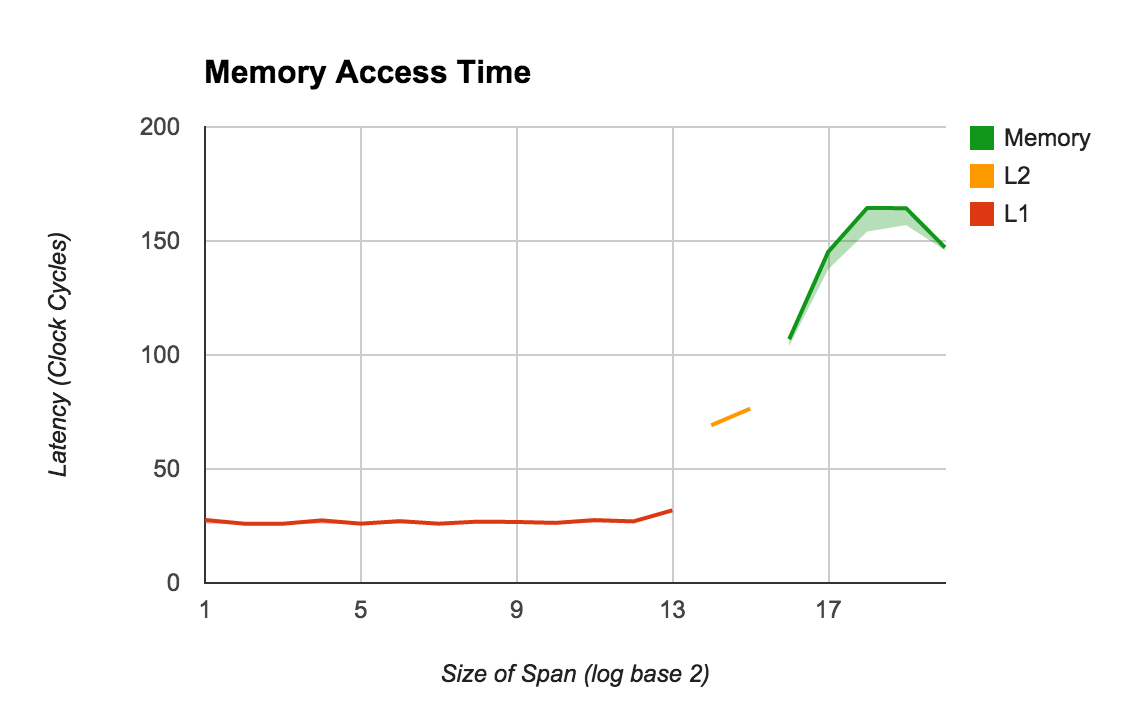
\includegraphics[scale=.5]{experiments/exp_2_1_fig.png}
\caption{Cycle count for memory read latency vs span size.  
Different memory regimes are labeled by color.  +/- 1 standard deviation highlighted by shading.}
\end{figure}

\newpage

\subsubsection{Bandwidth}Next we measure memory bandwidth: the number of bytes readable and writable per clock cycle.  
To measure this we allocate a block of memory of $2^{20}$ bytes, shown to be sufficiently large to use memory rather than cache.
We then write the value 1 into every byte in the span and measure the total time and divide by the number of bytes written.
To measure read bandwidth we repeat the write experiment but read/sum all the values written into the span.
To improve performance we unroll the writing and reading loop 16 times which should fully occupy the hardware scheduler.

We expect each access within the a cache line to be the same as an access to the l1 cache and each cahce line to have one main memory access.  Thus we expect a total latency of (150*1 + 25*15) = 525 time per cache line or 0.03 bytes accessed per cycle.  

Table \ref{tab:exp_2_2} shows our read and write bandwidth.  The read and write bandwidth are both about double our predicted bandwidth.  This is probably accounted for by the chip fetching multiple bytes at once.  A better experiment may use 16 or 32 bit integers rather than 8 bit bytes.  An interesting result is that write bandwidth is a bit higher than read.  It is likely that this is caused by write grouping writing large chunks to memory once the buffers are full. 

\begin{table}[h]
\label{tab:exp_2_2}
\begin{tabular}{|l|l|}
\hline
Type  & Bandwidth        \\\hline
Write & 0.08 Bytes/Cycle \\\hline
Read  & 0.05 Bytes/Cycle \\ \hline
\end{tabular}
\end{table}

\newpage

\subsubsection{Page Fault}To measure the page fault latency we generate a file containing 4MB of data from {\tt /dev/random}, since the page size is 4KB this corresponds to 1000 pages of data.  
We then memory map this file and then measure the latency of reading the first byte of each page.  
This corresponds to a page fault since the memory makes a block of memory and sets the file on disk to function as it's swapped page source.
Thus when we request a byte from the region which has not been brough into memory it is the same as a page fault.
In our later disk experiments, sequential reading of disk blocks, which have the same size and access pattern as we see in this experiment, have a mean latency of 250,000 cycles per block.
Since the access pattern is similar to our access pattern here, we expect similar performance; however, a common myth is that memory mapping (as used here) is faster than reading (as used in the disk experiments) due to page faulting using a better system compared to disk io.
Thus our estimate is likely a bit over.

Our experiment showed 150,000 cycles per page fault with a standard deviation of 33,000 cycles.
As expected, this is slightly faster than the performance of regular disk io.
However, it is within the same order of magnitude.

\newpage

\subsubsection{Miscellaneous: TLB miss}We decided that, in addition to the previous experiments, it was necessary to measure the time taken to service a TLB miss. This is important because during the memory measurement experiments, the set of experiments reading short stretches of data will consistently hit the TLB, whereas eventually, reading longer stretches consistently misses it. While our memory experiments currently do not take these behaviors into considerations, we will incorporate them into future experimental analysis.
\newline
\newline
Unfortunately, the TLB is fairly complicated on this architecture; there is a microTLB for data, as well as one for instructions, and a main TLB. Together, these contain about 80 mapping entries. For simplicity, we measured a complete TLB miss $-$ a miss on both the microTLB and the main TLB.
\newline
\newline
To do this, wrote one experiment which simply read the same variable over and over into a register. This one is guaranteed to hit the TLB and the data in the L1 cache. The trick is, how do we read data from L1 cache while missing the TLB? Our solution was to read different pages from memory until the TLB was flushed, but to make sure the page offset of the address read on each page had a different cache line tag than the variable we wanted to measure. This way, we would be sure to avoid evicting the variable from cache. After flushing the TLB, we read the variable of interest, (hopefully) missing the TLB entirely, but hitting the L1 cache. Taking the difference of these measurements should give us the TLB miss time.
\newline
\newline
Below is the code for the TLB hit experiment:
\begin{verbatim}
unsigned long measure() {
  // make sure v in cache
  v = 0;

  // load v's label into r4
  asm volatile("ldr r4, .L18");
  GET_HIGH(start);
  //load v's data into r4
  asm volatile("ldr r4, [r4]");
  GET_HIGH(end);
  return end - start;
}
\end{verbatim}

\newpage

\noindent Now, the code for the TLB miss experiment:
\begin{verbatim}
unsigned long measure() {
  //dyn is allocated on the heap
  //guaranteed to be on different page than tlb variable
  //load *dyn into cache
  *dyn = 0;

  //flush tlb, keep dyn in cache
  //alttag is a page offset with a different cache-line-
  //tag than *dyn
  char *s = start_page + alttag;
  for(int i = 0; i < TLB_ENTRIES; ++i) {
    // put *s's page in TLB
    *s = *s;
    s+=PAGE_SIZE;
  }

  //load dyn's label into r4
  asm volatile("ldr r4, .L22");
  //load dyn data into r4
  asm volatile("ldr r4, [r4]");
  GET_HIGH(start);
  //load *dyn data into r4
  asm volatile("ldr r4, [r4]");
  GET_HIGH(end);

  return end - start;
}
\end{verbatim}

\noindent The results are as follows: Hitting the TLB incurs 14 cycles; missing it appears to incur 96.8 cycles, with a standard deviation of 28 cycles. The latter measurement is certainly inaccurate. The most frequent cycle counts were 22 and 107. 107 probably represents a complete TLB miss, whereas 22 probably represents a microTLB miss and a main TLB hit. Because we are not able to control whether a page entry is loaded into the microTLB or the main TLB, this is not really the fault of our experiment, and we can safely assume that a memory read after a complete TLB miss takes 107 cycles. 

\newpage

\printbibliography

\end{document}